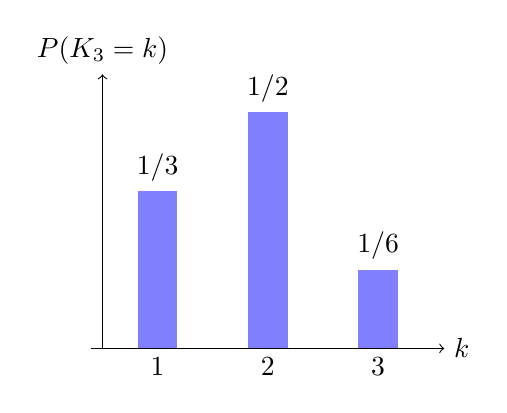
\begin{tikzpicture}[x=1.4cm,y=6cm]
\draw[->] (.4,0)--(3.6,0) node[right] {$k$};
\draw[->] (.5,0)--(.5,.58) node[above] {$P(K_3=k)$};
\foreach \k/\h/\lab in {1/.333333/{1/3},2/.5/{1/2},3/.166667/{1/6}}{
\fill[blue!50] (\k-.18,0) rectangle (\k+.18,\h);
\node[above] at (\k,\h) {$\lab$};
\node[below] at (\k,0) {$\k$};}
\end{tikzpicture}
